\begin{figure}[ht]
    \centering
    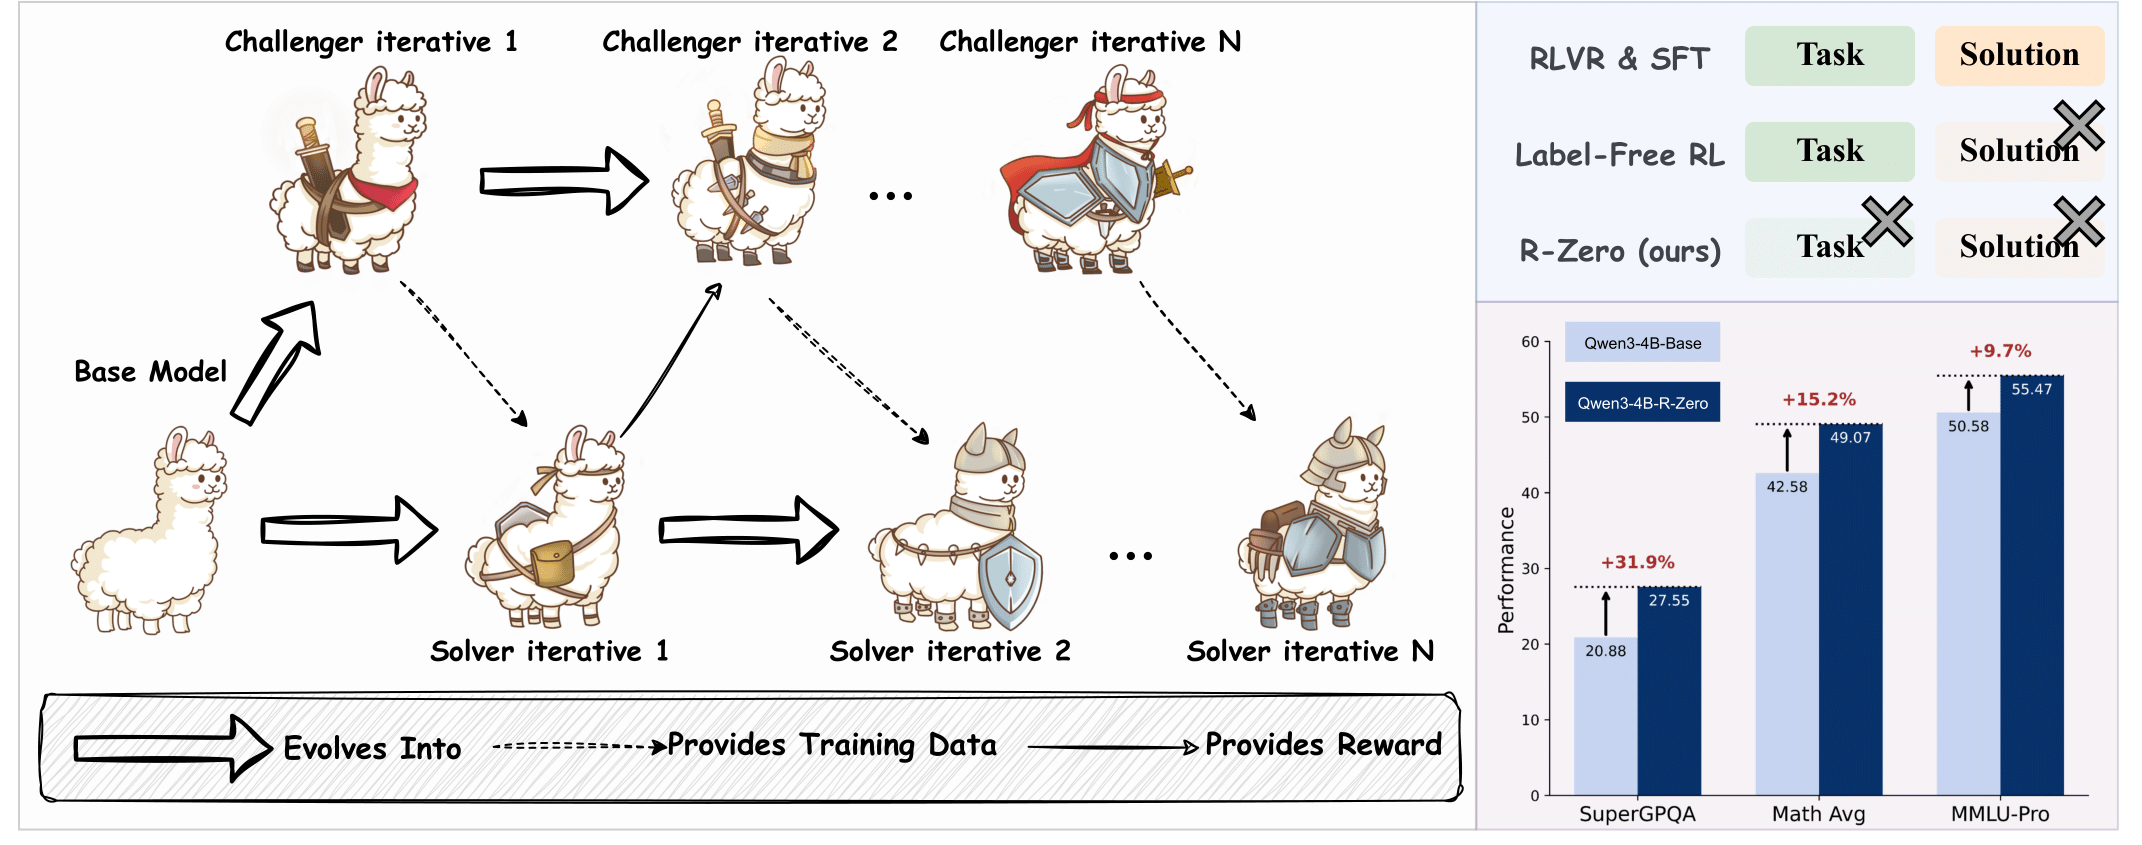
\includegraphics[width=0.95\linewidth]{figures/rebuttal.drawio-1.png}
    \caption{(Left): \textbf{\method{}} employs a co-evolutionary loop between Challenger and Solver. (Right): \textbf{\method{}} achieves strong benchmark gains without any pre-existing tasks or human labels.}
    \label{fig:abstract}
\end{figure}
\section{Introduction}



Self-evolving Large Language Models (LLMs) represent a promising frontier for advancing language intelligence. By autonomously generating, refining, and learning from their own experiences, these models provide a scalable pathway toward artificial superintelligence~\citep{Tao2024ASO,tan2024large}. 
A critical requirement for training such self-evolving LLMs is access to large volumes of expertly curated tasks and labels, which serve as supervision signals for fine-tuning or reinforcement learning with verifiable rewards (RLVR)~\citep{Shao2024DeepSeekMathPT,DeepSeekAI2025DeepSeekR1IR}. 
However, relying on human annotators to create these tasks and labels is not only costly, labor-intensive, and difficult to scale, but also presents a fundamental bottleneck to advancing AI toward capabilities that could eventually surpass human intelligence~\citep{Su2025CrossingTR,Zhao2025AbsoluteZR}.
% This underscores the needfor a new paradigm that begins to explore possibilities beyond the constraints of human-designed tasks and prepares for a future in which AI systems may surpass human intelligence.
% A prime example of this strategy is Reinforcement Learning with Verifiable Rewards (RLVR)~\citep{Lambert2024TLU3P}, a method now widely used for improving reasoning in domains like mathematics~\citep{Shao2024DeepSeekMathPT} and coding~\citep{Shi2025MobileGUIRLAM,Zhu2025CodeVR1RV} without relying on annotated thinking processes. 
% Despite its success, this method's reliance on human supervision remains substantial, as it still requires both a large collection of high-quality problems and their corresponding ground-truth answers for verification~\citep{Su2025CrossingTR}.

% Through self-evolution, AI has achieved superhuman performance in a series of increasingly complex but consistently well-defined games -- from the perfect information of Go~\citep{Silver2017MasteringTG} to the strategic depths of StarCraft II~\citep{Vinyals2019GrandmasterLI} and the team-based coordination of Dota 2~\citep{Berner2019Dota2W}. 
% However, in natural language, which lacks such clear ``win conditions'', applying this principle has required a strategic focus on tasks with at least a verifiable final outcome.
% However, applying this principle to natural language is more challenging, since there are no clear ``win conditions''. As a result, efforts have focused on tasks with outcomes that can be verified~\citep{DeepSeekAI2025DeepSeekR1IR}.

To reduce dependence on human-curated data, self-generated and label-free methods have been proposed to eliminate the need for explicit supervision. In particular, label-free RL derives reward signals directly from the model's own outputs, such as sequence-level confidence scores~\citep{Li2025ConfidenceIA, Prabhudesai2025MaximizingCA, Huang2025EfficientTestTimeScalingSelfCalibration} and output entropy~\citep{Agarwal2025TheUE,Cheng2025ReasoningWE}.
However, despite removing the need for explicit labels, label-free methods still relies on a pre-existing corpus of tasks, which limits its scalability in truly self-evolving settings.
% While these innovations successfully removed the dependency on annotated solutions or labels, a fundamental bottleneck persists across all existing paradigms: they all presuppose the existence of a large, pre-existing corpus of tasks (the problems themselves). 
% To further reduce this data dependency, more recent "label-free" approaches take another step by eliminating the need for ground-truth answers. These methods generate reward signals directly from the model’s own outputs, using heuristics like sequence-level confidence scores~\citep{Li2025ConfidenceIA, Prabhudesai2025MaximizingCA}, consistency across multiple solutions~\citep{Zhang2025ConsistentPL, Zuo2025TTRLTR, Zhang2025RightQI}, or minimizing output entropy~\citep{Agarwal2025TheUE, Cheng2025ReasoningWE}. While these innovations successfully removed the dependency on annotated solutions or labels, a fundamental bottleneck persists across all existing paradigms: they all presuppose the existence of a large, pre-existing corpus of tasks (the problems themselves). 
On the other side, self-challenging approaches train LLMs on tasks generated by the models themselves~\citep{Zhou2025SelfChallengingLM,Wang2025CoEvolvingLC,Zhao2025AbsoluteZR}.
While promising, many of these methods rely on external code executors to ensure that the synthesized tasks are both feasible and verifiable. However, in domains that lack an explicit verification oracle, such as open-ended reasoning, ensuring the quality and correctness of self-generated data remains a significant challenge.

In this paper, we propose \method{}, a framework for training reasoning LLMs that can self-evolve from zero external data.
In \method{}, a single base model is initialized with two roles -- a \textbf{Challenger} and a \textbf{Solver} that are independently optimized but \textbf{co-evolve} throughout the RL process.
% built on the co-evolution of a \textbf{Challenger} and a \textbf{Solver}, which are both initialized from the same base model. 
During co-evolving, the Challenger is rewarded for generating tasks targeted to be at the edge of Solver's current abilities, while the Solver is rewarded for solving increasingly challenging tasks posed by the Challenger. Framework details are provided in Section \ref{sec:method}, but briefly, in the Challenger training phase, the Challenger is trained via Group Relative Policy Optimization (GRPO)~\citep{Shao2024DeepSeekMathPT} to generate difficult questions. The reward signal is derived from the uncertainty for the frozen Solver, which is measured by the self-consistency of its multiple generated answers. In the Solver training phase, the Solver is fine-tuned with GRPO on a filtered set of these challenging questions generated by the now-frozen Challenger, using the pseudo-labels voted by itself. This entire process repeats, creating a self-evolving cycle that operates without any human intervention.

Our experiments demonstrate that \method{} is a model-agnostic framework, consistently and iteratively improving the reasoning abilities of different backbone LLMs. For example, Qwen3-4B-Base model's average score on math benchmarks increased by a significant \textbf{+6.49} points after three iterations of self-evolution. Moreover, the reasoning skills learned through our math-focused questions can generalize to complex general-domain tasks, with models trained using \method{} showing significant improvements on general domain reasoning benchmarks like MMLU-Pro~\citep{Wang2024MMLUProAM} and SuperGPQA~\citep{Team2025SuperGPQASL}. Our further analysis finds that \method{} can act as a mid-training method, as models first improved by our method achieve higher performance after fine-tuned on labeled data.
In addition, we provide an in-depth analysis that validates our framework's components, demonstrates its synergy with supervised fine-tuning, and characterizes the co-evolutionary dynamics to identify both strengths and limitations, offering insights for future research.
